\documentclass{article}
\usepackage{graphicx}
\begin{document}
\noindent
\begin{tabular}{lr}
CHALMERS TEKNISKA H\"OGSKOLA &Tuesday 16th December, 2008.\\
Dept. of Computer Science and Engineering & Programming Paradigms\\
John Hughes                  & DAT120(CTH) / DIT330(GU) \\
\end{tabular}

\vspace{2.5cm} \noindent
\begin{center} {\LARGE
Exam in Programming Paradigms}
\end{center}

\vspace{1.5cm}

\noindent
Tuesday 16th December, 2007, EM.\\
Lecturer: John Hughes, tel 070 756 3760.
\vspace{1cm}

\noindent
Permitted aids:\\
English-Swedish or English-other language dictionary.

There are five questions, one on each paradigm, worth 12 points each
for a total of 60 points. 24 points is required to pass (grade 3), 36
points is required for grade 4, and 48 points is required for grade 5.

%\newcommand{\comment}[1]{}
\newcommand{\comment}[1]{\marginpar{#1}}

\newpage

\section{Imperative Programming [12 points]}

\begin{enumerate}
\item (Parameter passing.) 
\hfill{\textbf{[4 points]}}
\begin{enumerate}
\item Given  the following program:

{\small
\begin{verbatim}
int i;
int a[2];
void p(int x, int y) {
    x++;
    i++;
    y++;
}
int main () {
    a[0] := 1;
    a[1] := 1;
    i := 0;
    p(a[i],a[i]);
    print ("a[0] = ", a[0]);
    print ("a[1] = ", a[1]);
    return 0;
}
\end{verbatim}
}

For each of the following methods of parameter passing,
draw the activation record of the subroutine \texttt{p} at the time when
the parameters are passed. Also give the output of above program
in each of the cases

\begin{enumerate}\itemsep=0.0cm
\item Call-by-reference
\item Call-by-value
\item Call-by-result
\item Call-by-value-result; if the return address is computed...
\begin{enumerate}\itemsep=0.0cm
\item early (beginning of the call)
\item for x and y separately (before and after i++)
\item late (when the call returns)
\end{enumerate}
\end{enumerate}
 (\textbf{2p.})
\item Consider the following definition of the 
subroutine \texttt{sum}: 

{\small 
\begin{verbatim}
int sum (by-name int a, by-name int index, int size)
{
    int tmp = 0;
    for (index = 0; index < size; index++)
    {
        tmp +=a;
    }
    return tmp;
}
int x[10];
...
int result =  sum(?,?,10);              //  (*)   
\end{verbatim}
}
 Assume the integer array \texttt{x[10]}, of size 10, is appropriately
initialized. Demonstrate the use of \textit{call-by-name} in the invocation of
\texttt{sum} (see the line marked (*)) by filling in the
proper actual arguments so that the call to \texttt{sum} computes
the sum of all elements from \texttt{x[0]} to \texttt{x[9]}. 
Introduce auxiliary variables where necessary. (\textbf{2p.})
\\
\end{enumerate} 

\item (Immutability.) \hfill{\textbf{[4 points]}}
\\
The \texttt{String} concatenation operator \texttt{+} in the Java
language is specified as follows:


\begin{quote}
(JLS, 15.18.1) String Concatenation Operator +

``If only one operand expression is of type String, then string conversion is performed on the other operand to produce a string at run time. The result is a reference to a String object (newly created) that is the concatenation of the two operand strings. The characters of the left-hand operand precede the characters of the right-hand operand in the newly created string. If an operand of type String is null, then the string ``null" is used instead of that operand.''
\end{quote}

 Given the following class 
in the Java language: 
{\small 
\begin{verbatim}
class GoodMorning 
{
   public static void appendMorning (String t)
   {
       t = t + "Morning";
   }
   public static void main(String [] args)
   {
       String s = "Good ";
       appendMorning(s);
       System.out.println(s);
   }
}
\end{verbatim}
}
\begin{enumerate}
\item
The specification of the string concatenation operator allows 
the Java String class to be \textit{immutable}. Read the
specification above carefully and determine \textit{where} in the specification
immutability comes into play. Give the  phrase(s) literally, as used in 
the wording of the specification. (\textbf{2p.})
\item 
What does the program print? 
Draw a snapshot of the stack of activation records (``run-time stack'')
when the string concatenation operator \texttt{+} is invoked and the parameter is passed;
draw another snapshot directly after \texttt{+} has returned. 
Use the snapshots to explain. (\textbf{2p.})
\end{enumerate}


\item (Scoping.)
\hfill{\textbf{[4 points]}}
\\
Assume a for-statement in a Java-like language, that is, of the form
 
\begin{center}
  \textbf{for} (ForInit; Expression; ForUpdate) Statement.
\end{center}
Further assume the scope of a local variable declared in the 
\textit{ForInit} part of a 
for-statement includes all of the following:
\begin{itemize}
    \item Its own initializer.
    \item Any further declarators to the right in the \textit{ForInit} 
          part of the for-statement.
    \item The \textit{Expression} and \textit{ForUpdate} parts of the 
          for-statement.
    \item The contained \textit{Statement}. 
\end{itemize}

Your task:
\begin{enumerate}
\item There are other scopes besides for-loops. Give the names of two
additional examples of scopes. 
(\textbf{1p.})
\item Consider the following three snippets of for-loops. For each snippet, 
determine whether it compiles or fails with a scoping-related error
(make no additional assumptions about the variable \texttt{i}). In case
of an error, mark its position in the snippet and give a useful error message
that a compiler could provide. (\textbf{3p.})
{\small
\begin{verbatim}
//  Snippet 1
for (int i = 0; i < 10; i++) {
      ... 
}
i = 5;      

//  Snippet 2 
int i = 5;
for (int i = 0; i < 10; i++) {   
    ...
}
    
// Snippet 3
for (int i = 0; i < 10; i++) {
    ...
}

for (int i = 0; i < 10; i++) { 
    ...
}
    
\end{verbatim}
}


\end{enumerate}
\end{enumerate}

\newpage
\section{Object-Oriented Programming [12 points]}

\begin{enumerate}
\item (Smalltalk.) 
\hfill{\textbf{[4 points]}}
\\
Consider the message \texttt{lineCount} in the Smalltalk class \texttt{String}.

{\small 
\begin{verbatim}
lineCount 
"Answer the number of lines represented by the receiver, where 
every cr adds one line." 
| cr count |                                               "(1)"
cr := Character cr.                                        "(2)"
count := 1 min: self size.                                 "(3)"
self do: [:c | c == cr ifTrue: [count := count + 1]].      "(4)"
^ count                                                    "(5)"

\end{verbatim}
}
\begin{enumerate}
\item What do the bars in line (1) and the period (in lines 2-4) 
mean? Give the technical term for each. (\textbf{1p}.)
\item In lines (3) and (4): determine all messages, and 
for each message determine the receiver object and all 
argument object(s). For readability,
provide your answers in tabular form
\begin{center}
\begin{tabular}{lll}
Message & Receiver & Argument(s) \\ \hline
...     & ...      & ...     \\
\end{tabular}
\end{center}   (\textbf{3p}.)
\end{enumerate} 

\item (Algebraic specification.)  \hfill{\textbf{[4 points]}}
\\
Assume an abstract data type Natural with 4 
operations: zero,
succ, add, and is-zero. Consider zero and succ as constructors.
%is-zero as observer.
\begin{enumerate}
\item Provide an appropriate signature. (\textbf{2p}.)
\item Provide the appropriate axioms that capture the intuitive 
understanding of zero, succ, addition, and is-zero for natural numbers.
Your axioms should allow one to show the identity

\begin{center}
{add(succ(succ(zero)), succ(zero)) = succ(succ(succ(zero)))}.
\end{center} 
(\textbf{2p.})
\end{enumerate}
\newpage
\item (Polymorphic methods, static and dynamic binding.)
\hfill{\textbf{[4 points]}}
\\
Many object-oriented languages provide keywords with which  
users can control whether a method gets bound dynamically or
statically; in the pseudo language used below, \texttt{virtual}
indicates dynamic binding. 

{\small 
\begin{verbatim}
class A {
     public non-virtual void f() { print( "A.f "); }
     public virtual void g()     { print( "A.g "); }
     public non-virtual void h() { f(); g(); }
    
}
class B inherits A {
     public non-virtual void f() { print( "B.f "); }
     public virtual void g()     { print( "B.g "); }
}
int main() {
      A a;
      B b;
      // initialization of a,b
      a.h();
      b.h();
      a = b;
      a.h(); 
}
\end{verbatim}
}
\begin{enumerate}
\item What gets printed if a,b have value types?  (\textbf{2p}.)
\item What gets printed if a,b have reference types?  (\textbf{2p}.)
\end{enumerate}
\end{enumerate}

\newpage

\section{Functional Programming [12 points]}

\begin{enumerate}
\item

Given
\begin{eqnarray*}
\mbox{\it inc}&=&\lambda x.~x+1\\
\mbox{\it twice}&=&\lambda f.~\lambda x.~f~(f~x)
\end{eqnarray*}
use $\beta$-conversion to simplify the following $\lambda$-expression as far as possible:
\[
\mbox{\it twice}~\mbox{\it twice}~\mbox{\it inc}~0
\]
Show each step in your answer.
\comment{1 point}


\item
{\em Church numerals} are a representation of natural numbers as
$\lambda$-expressions, where the $\lambda$-expression $\lambda
f.~\lambda x.~f^n(x)$ represents the natural number $n$. For brevity,
we shall write this $\lambda$-expression as $\hat{n}$. Define
$\lambda$-expressions {\it suc} and {\it add} that implement the
successor and addition functions, such that
\begin{eqnarray*}
\mbox{\it suc}~\hat{n}&=&\widehat{n+1}\\
\mbox{\it add}~\hat{m}~\hat{n}&=&\widehat{m+n}
\end{eqnarray*}
(Note that defining {\em suc} as $\lambda \hat{n}.~\widehat{n+1}$
would make no sense---$\hat{n}$ stands for a $\lambda$-expression, not
a variable name, and indeed, no ``hats'' ($\hat{~}$) should appear in
your answer).
\comment{2 points}


\item
Suppose the Haskell type \verb!Set a! represents a {\em set} of values
of type \verb!a!.
\begin{enumerate}
\item
Suggest suitable types for the functions \verb!insert! and
\verb!delete!, where \verb!insert a s! inserts an element \verb!a!
into the set \verb!s!, and \verb!delete a s! removes an element
\verb!a! from a set \verb!s!.
\comment{1 point}

\item
What will the value of the following expression be, given that
\verb!s! is the set $\{1,2\}$? You may write set values informally
using the usual mathematical notation $\{x_1, x_2, x_3\dots\}$.
\begin{verbatim}
(delete 2 s, insert 3 s)
\end{verbatim}
\comment{1 point}

\end{enumerate}

\item
Sets can be implemented by {\em ordered binary trees}, in which each
node is either a {\em leaf}, or a {\em branch} containing a left
sub-tree, an element, and a right sub-tree, with the invariant that
all the elements in the left sub-tree are less than the element in the
branch node, and all the elements in the right sub-tree are greater
than it. Ordered binary trees can be represented by the following
Haskell type:
\begin{verbatim}
data Set a = Leaf | Branch (Set a) a (Set a)
\end{verbatim}
The following function inserts a new element into such a
tree, in the correct position.
\begin{verbatim}
insert a Leaf = Branch Leaf a Leaf
insert a (Branch l b r) =
  if a==b then Branch l b r
  else if a < b then Branch (insert a l) b r
  else Branch l b (insert a r)
\end{verbatim}
\begin{enumerate}
\item
Given the definition
\begin{verbatim}
t = insert 1 (insert 4 (insert 2 Leaf))
\end{verbatim}
then the following diagram illustrates the value of
\verb!t!.

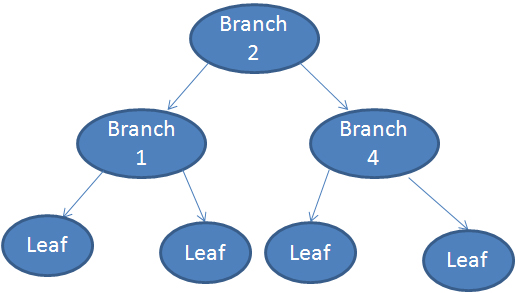
\includegraphics[width=6cm]{tree.jpg} 

Copy this diagram, and {\em in the same diagram} draw the data-structure
returned by \verb!insert 3 t!. Make sure you accurately represent any
sharing between old and new trees.
\comment{1 point}


\item
In your diagram, mark the nodes that will be reclaimed by the garbage
collector assuming that there are no references to \verb!t!, but there
is a reference to the result of \verb!insert 3 t!.
\comment{1 point}


\item
Define a function \verb!delete!, which deletes an element from a tree.
\comment{3 points}


{\em Hint:} you will find you need a function to join together the
left and right subtrees of a branch-node into a single tree. You can
use the following function to do this:
\begin{verbatim}
join Leaf t = t
join (Branch l b r) t = Branch l b (join r t)
\end{verbatim}
There is no need to repeat this definition in your answer.

\item
Suppose the function
\begin{verbatim}
setElements :: Ord a => Set a -> [a]
\end{verbatim}
returns a sorted list of the elements of a set. Write a {\em
  QuickCheck property} that uses an ordered list of elements as a {\em
  model} to test the \verb!insert! function.  You may assume that
QuickCheck can already generate random \verb!Set! values (so you do
not need to define a generator for \verb!Set!s), and you may use the
function \verb!List.insert x xs! that inserts an element \verb!x! into
an ordered list \verb!xs! in the correct position.  \comment{2 points}



\end{enumerate}




\end{enumerate}

\newpage
\section{Concurrency Oriented Programming [12 points]}

Study the following Erlang code, which implements a simple {\em generic server}.
\begin{verbatim}
start_server(M) ->
  register(M,spawn(fun() -> server(M,M:init()) end)).

server(M,S) ->
  receive
    {Pid,Msg} ->
      {Reply,NewS} = M:handle(S,Msg),
      reply(M,Pid,Reply),
      server(M,NewS)
  end.

reply(M,Pid,Msg) ->
  Pid ! {M,Msg}.

rpc(M,Msg) ->
  M ! {self(),Msg},
  receive {M,Reply} -> Reply end.
\end{verbatim}

\begin{enumerate}

\item
What do the following notations mean?
\begin{enumerate}
\item \verb,Pid ! Msg,
\item \verb!receive Msg -> ... end!
\end{enumerate}
\comment{2 points}

\item 
Erlang does not provide locks to protect shared data from simultaneous
modification by two or more concurrent processes. What prevents Erlang
processes from corrupting shared data?
\comment{1 point}

\item
Suppose we want to use the generic server above to create a server
that implements a {\em variable}, with initial value zero, handling
requests \verb!read! to read the variable's value, and
\verb!{write,X}! to set the variable's value to \verb!X!. For example,
we might increment the value held in the variable using the following
code in a client:
\begin{verbatim}
N = rpc(variable,read),
rpc(variable,{write,N+1})
\end{verbatim}
Write definitions of the callback functions \verb!init! and
\verb!handle! to implement this behaviour.
\comment{2 points}

\item
When a client tries to increment the variable's value using the code
above, there is a risk that a different client might change the
variable's value between the read and the write. We might therefore
wish to add two new requests to the server's repertoire: \verb!lock!
  and \verb!unlock!, so that the code above can be written as
\begin{verbatim}
rpc(variable,lock),
N = rpc(variable,read),
rpc(variable,{write,N+1}),
rpc(variable,unlock)
\end{verbatim}
with the effect that the server only accepts requests from this client
between the lock and the unlock. Show how to {\em modify the generic
  server} so that {\em all} servers implemented using it support the
\verb!lock! and \verb!unlock! requests.
\comment{2 points}

{\em Hint:} you can write code such as
\begin{verbatim}
receive 
  {Pid,{write,X}} when X>0 -> 
    ... 
end
\end{verbatim}
to accept a message only when a certain condition holds.

\item
What happens to requests from {\em other} clients, which are sent
while the lock is held?
\comment{1 point}

\item
What is the effect of {\em linking} two Erlang processes?
\comment{1 point}

\item
Show how to modify your generic-server-with-locking, so that if a client
crashes while holding the lock, then
\begin{itemize}
\item the lock is released, so that other clients can use the server,
\item the {\em state} of the server is restored to the value it had
  when the lock was last claimed---so that a client which crashes
  while holding the lock has no visible effect, as far as other
  clients are concerned.
\end{itemize}
\comment{3 points}

\end{enumerate}

\newpage
\section{Logic Programming [12 points]}

\begin{enumerate}
\item
What is the result of unification of the following pairs of terms? In
each case, state whether or not unification succeeds, and if it
succeeds, give the values bound to the variables.  \comment{2 points}

\noindent
\begin{minipage}{0.5\textwidth}
  \begin{enumerate}
  \item
  \verb![X|Xs]! and \verb![1,2,3]!
  \item
  \verb![X,2]! and \verb![1,Y]!
  \item
  \verb![A,A]! and \verb![1,B]!
  \item
  \verb![A,B]! and \verb![1,2,3]!
  \end{enumerate}
\end{minipage}
\begin{minipage}{0.5\textwidth}
  \begin{enumerate}
  \item
  \verb|true| and \verb!X=1! and \verb!Xs=[2,3]!
  \item
  \verb|true| and \verb!X=1! and \verb!Y=2!
  \item
  \verb|true| and \verb!A=B=1!
  \item
  \verb|false|
  \end{enumerate}  
\end{minipage}

\item
Given the clauses
\begin{verbatim}
mem(X,[X|Xs]).
mem(X,[Y|Xs]) :- mem(X,Xs).
\end{verbatim}
what will Prolog display in response to these queries? Make sure to
include all the solutions Prolog will find.
\comment{3 points}

\noindent
\begin{minipage}{0.5\textwidth}
  \begin{enumerate}
  \item \verb!mem(X,[]).!
  \item \verb!mem(X,[1,2,3]).!
  \item \verb!mem(1,X).!
  \end{enumerate}
\end{minipage}
\begin{minipage}{0.5\textwidth}
  \begin{enumerate}
  \item \verb!false!
  \item \verb!true! and (\verb!X=1! or \verb!X=2! or \verb!X=3!)
  \item \verb!true! and \verb!X=[...,1,...]!
  \end{enumerate}
\end{minipage}

\item
Using no more than two clauses, define a predicate \verb!del(X,Xs,Ys)!
which holds when \verb!X! is an element of the list \verb!Xs!, and
removing one \verb!X! from \verb!Xs! leaves the list \verb!Ys!. For
example, given the query \verb!del(2,[1,2,3],Ys)!, Prolog should reply
with \verb!Ys = [1,3]!.
\comment{2 points}

\begin{verbatim}
del(X,[X|Xs],Xs).
del(X,[Y|Xs],[Y|Ys]) :- del(X,Xs,Ys).
\end{verbatim}

\item
What solutions will Prolog find for the queries
\comment{2 points}

\noindent
\begin{minipage}{0.35\textwidth}
  \begin{enumerate}
  \item
  \verb!del(1,[1,2,1],Ys).!
  \item
  \verb!del(3,Xs,[1,2]).!
  \end{enumerate}
\end{minipage}
\begin{minipage}{0.65\textwidth}
  \begin{enumerate}
  \item
  \verb!Ys=[2,1]! or \verb!Ys=[1,2]!
  \item
  \verb!Xs=[3,1,2]! or \verb!Xs=[1,3,2]! or \verb!Xs=[1,2,3]!
  \end{enumerate}
\end{minipage}

\item
Study the following clauses, which define the predicate
\verb!reverse(Xs,Ys)! that holds if the lists \verb!Xs! and
\verb!Ys! are each other's reversal.  
\begin{verbatim}
reverse([],[]).
reverse([X|Xs],Ys) :- reverse(Xs,Zs), append(Zs,[X],Ys).
\end{verbatim}
This uses the \verb!append! predicate from the lectures:
\begin{verbatim}
append([],Ys,Ys).
append([X|Xs],Ys,[X|Zs]) :- append(Xs,Ys,Zs).
\end{verbatim}
\begin{enumerate}
\item
Both of the queries \verb!reverse([1,2,3],Xs)! and
\verb!reverse(Xs,[1,2,3])! find the solution \verb!Xs = [3,2,1]!, but
one of them falls into an infinite loop if we ask for more
solutions. Which query can fall into an infinite loop?
\comment{1 point}

The second (\verb!reverse(Xs,[1,2,3])!) will loop endlessly, because
the code only specifies that \verb!Xs1! should be unified with \verb![X|Xs2]!,
and that \verb!Ys! should be unified with \verb![1,2,3]!. The recursive
use of \verb!reverse! then performs a similar unification, without making
progress.
\item
Using no more than three clauses, give a definition of the
\verb!reverse! predicate which does not fall into a loop in either of
these cases.
\comment{2 points}

\begin{verbatim}
reverse([],[]).
reverse(Xs,[Y|Ys]) :- nonvar(Ys), !, reverse(Ys,Zs), append(Zs,[Y],Xs).
reverse([X|Xs],Ys) :- reverse(Xs,Zs), append(Zs,[X],Ys).
\end{verbatim}

\end{enumerate}

\end{enumerate}

\end{document}
